\documentclass{scrarticle}                % use [twocolumn] option for two-column layout

% packages.tex

% ---------------- used packages for LaTeX Document

\usepackage[english, german]{babel}                 % Language support for English and German. Handles language-specific typographic rules and hyphenation.
\usepackage{listings}                               % Provides support for including source code in your document. Customizable for various programming languages.
\usepackage{caption}                                % customised captions in floating environments
\usepackage{xcolor}                                 % Provides color support. Allows for color definitions and styling, including colored text, tables, and code.
\usepackage{array}                                  % Enhances the array and tabular environments with additional features like column definitions and customizations.
\usepackage{graphicx}                               % Improves handling of graphics. Allows for easy inclusion, scaling, and rotation of images.
\usepackage{tabularx}                               % Provides an extended tabular environment with more flexibility in defining table widths and column types.
\usepackage{booktabs}                               % For professional looking tables
\usepackage{amsmath}                                % Provides enhanced mathematical typesetting. Includes additional symbols, environments, and improved equation formatting.
\usepackage{tcolorbox}                              % Provides colored boxes for creating styled content blocks like notes, warnings, and examples.
\usepackage{fontawesome5}                           % Provides access to Font Awesome 5 icons for use in documents. Useful for adding symbols and icons to content.
\usepackage{pdfpages}                               % Allows for including external PDF files in the document. Useful for adding full-page PDFs, like appendices or reports.
\usepackage{pdflscape}                              % Provides landscape pages for PDF output. Allows individual pages to be rotated to landscape orientation.
\usepackage{subfiles}                               % Facilitates the use of subfiles in large documents. Allows for separate LaTeX files for different sections of a project.
\usepackage{csquotes}                               % Provides enhanced quote handling with support for different quotation styles and languages. Ensures correct typographic quotation marks.
\usepackage{pdflscape}                              % Provides landscape pages for PDF output. Allows individual pages to be rotated to landscape orientation.
\usepackage{lipsum}                                 % Generates placeholder text for testing. Useful for creating sample text for documents and templates.
\usepackage{hyperref}                               % Provides support for hyperlinks in the document. Allows for clickable links for references, URLs, and internal document links.
\usepackage{longtable}                              % Allows for tables that span multiple pages. Useful for large tables that do not fit on a single page.
\usepackage[backend=biber, style=ieee]{biblatex}    % Bibliography management. Uses Biber as the backend for processing bibliographic data and formats citations and references in IEEE style.
\usepackage{fancyhdr}                               % Headers
\usepackage{float}                                  % Improves the interface for defining floating objects such as figures and tables.
\usepackage{longtable}                              % larger tabular environment
\usepackage{hyperref}                               % Provides support for hyperlinks in the document. Allows for clickable links for references, URLs, and internal document links.

           % \usepackage{} statements
\newcolumntype{L}[1]{>{\raggedright\arraybackslash}p{#1}}  % Left-aligned column with fixed width
\newcolumntype{C}[1]{>{\centering\arraybackslash}p{#1}}    % Centered column with fixed width
\newcolumntype{R}[1]{>{\raggedleft\arraybackslash}p{#1}}   % Right-aligned column with fixed width

\setlength{\parindent}{0pt} % kein Einzug nach Absatz
% \setlength{\parindent}{15pt} % Standardmässiger Einzug
% \noindent % Temporär keinen Einzug

\usetikzlibrary{matrix, backgrounds} 

\newcommand\zeilenabstand{10pt} 

\def\GetNodeColumn(#1-#2-#3){#3}

\tikzset{vp/.style={circle, fill, inner sep=2pt}} 
\newcommand\verbindungslinie[4][10pt]{ 
  \node[#2, vp] at ([yshift=-.15*\zeilenabstand]#3.south) {};
  \edef\co{\noexpand\GetNodeColumn(#3)}
  \foreach[remember=\p as \lastp (initially #3)] \p in {#4} 
    \edef\cl{\noexpand\GetNodeColumn(\lastp)}
    \edef\cp{\noexpand\GetNodeColumn(\p)}
    \draw[ultra thick, #2, draw opacity=.4]
        ([yshift=-.15*\zeilenabstand,xshift={#1*(\co-\cl)}]\lastp.south) -- 
        ([yshift=-.15*\zeilenabstand,xshift={#1*(\co-\cp)}]\p.south) 
        node[vp] {}; 
}            % custom commands and environments
\addbibresource{references.bib}         % add .bib file - for examples see example folder

% ============================================================================== %
%                                   Margins                                      %
% ============================================================================== %

\usepackage[left=3cm, bottom=3cm, right=3cm, top=3cm]{geometry}

% ============================================================================== %
%                                     Header                                     %
% ============================================================================== %

\newcommand{\Abgabenummer}{4}

\pagestyle{fancy}
\fancyhf{}                              % empty all headers
\fancyhead[L]{Schlussbericht}           % top left
\fancyhead[C]{Team 10}                  % top middle
\fancyhead[R]{PREN 1}                   % top right
\fancyfoot[R]{\thepage}                 % pagenumber in footer

\fancypagestyle{nofooter}{
    \fancyhf{}                           % Leert Fusszeile und Kopfzeile
    \fancyhead[L]{Schlussbericht}        % Kopfzeile links
    \fancyhead[C]{Team 10}               % Kopfzeile Mitte
    \fancyhead[R]{PREN 1}                % Kopfzeile rechts
}

\begin{document}

% ============================================================================== %
%                                 Title Page                                     %
% ============================================================================== %

\begin{titlepage}
    \centering
    % \includegraphics[width=0.15\textwidth]{example-image-1x1}\par\vspace{1cm}
    {\scshape\LARGE Hochschule Luzern \par}
    \vspace{1cm}
    {\scshape\Large PREN 1 Team 10\par}
    \vspace{1cm}

    % Autoren zentriert
    {\scshape\large Julian Bischof\par}
    {\scshape\large Gabriel Buckland\par}
    {\scshape\large Sarangan Gopalachandran \par}
    {\scshape\large Yannick Merz\par}
    {\scshape\large Sandro Mösch\par}
    {\scshape\large Manuel Zihlmann\par}

    \vspace{1.5cm}
    {\huge\bfseries Schlussbericht PREN 1 \par}

    \vspace{1cm}

    \begin{figure}[H]
        \centering
        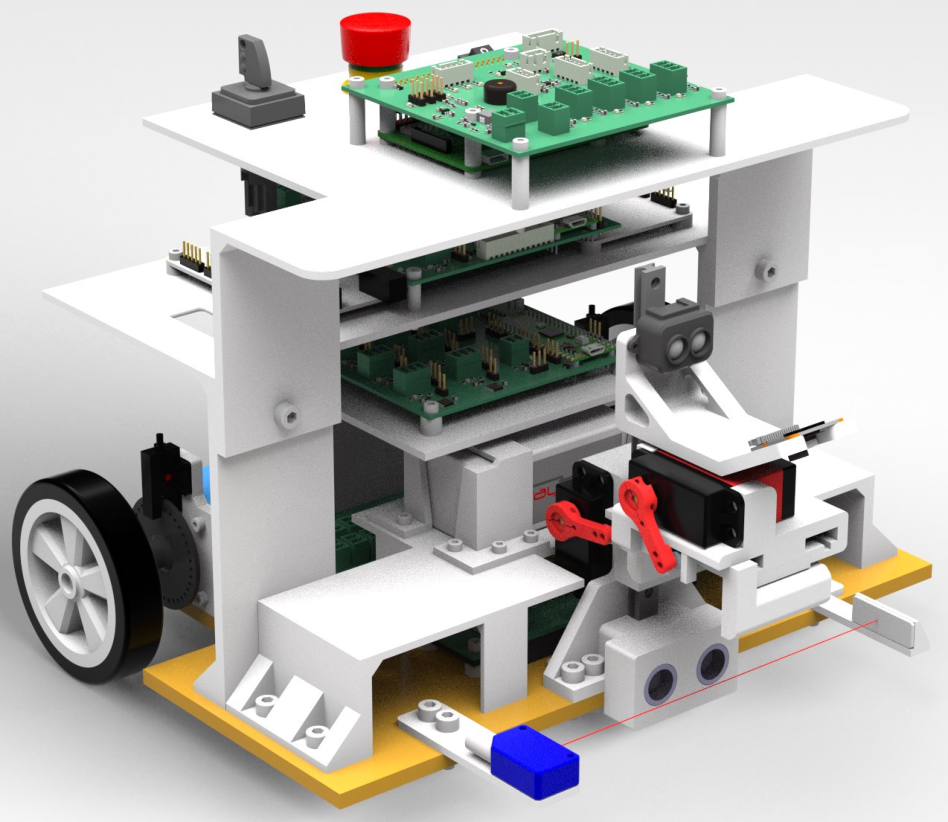
\includegraphics[width=0.85\textwidth]{Render_Baugruppe.pdf}
    \end{figure}

    \vfill
    % Bottom of the page
    {\large \today\par}
\end{titlepage}

\newpage

% ============================================================================== %
%                              Version History                                   %
% ============================================================================== %

\section*{Versionsverlauf}

\thispagestyle{nofooter}

\begin{longtable}{|p{2cm}|p{3cm}|p{3cm}|p{5cm}|}
    \hline
    \textbf{Version} & \textbf{Datum} & \textbf{Verfasser} & \textbf{Änderungen}                    \\
    \hline
    1.0              & 06.12.2024     & Team 10            & Erste Fassung                          \\
    \hline
    2.0              & 07.01.2025     & Team 10            & Abgabe der Schlussdokumentation PREN 1 \\
    \hline
    \caption{Versionsverlauf der Dokumentation}
\end{longtable}

\newpage

% ============================================================================== %
%                                Main Document                                   %
% ============================================================================== %

\subfile{./subfiles/Abstract.tex}
\thispagestyle{nofooter}
\newpage

\tableofcontents
\thispagestyle{nofooter}
\newpage

\setcounter{page}{1}

\subfile{./subfiles/Einleitung.tex}
\newpage

\subfile{./subfiles/Produktbeschreibung.tex}
\newpage

\subfile{./subfiles/Entwicklung_und_Dimensionierung.tex}
\newpage

\subfile{./subfiles/Projektmanagement.tex}
\newpage

\subfile{./subfiles/Nachhaltigkeit.tex}
\newpage

\subfile{./subfiles/Schlussdiskussion.tex}
\newpage

\subfile{./subfiles/Verzeichnisse.tex}
\newpage

\subfile{./subfiles/Anhang.tex}
\newpage

\end{document}

% ============================================================================== %
%                                   Examples                                     %
% ============================================================================== %

% ================================== Add Subfiles ============================== %

% \section{new Subfile}
% \subfile{./subfiles/subfile_template.tex}
% \newpage

% =============================  placeholder Texts ============================= %

% \lipsum[1-3] - creates first 3 paragraphs
% \lipsum[4]   - creates fourth paragraph

% ==================================== figures ================================= %

% \begin{figure}[h] % 'h' means here, placing the figure at the location in the text
%     \centering % Center the figure on the page
%     \includegraphics[width=0.5\textwidth]{example-image/path} % Adjust the width to 50% of text width
%     \caption{An example of a basic graphic} % Caption for the figure
%     \label{fig:example} % Label for referencing the figure
% \end{figure}

% % ---------- Include a graphic with specified width and height
% \begin{figure}[h]
%     \centering
%     \includegraphics[width=0.7\textwidth, height=0.5\textheight]{example-image}
%     \caption{Graphic with specific width and height}
%     \label{fig:size}
% \end{figure}

% % ---------- Scale the graphic to a specific percentage of its original size
% \begin{figure}[h]
%     \centering
%     \includegraphics[scale=0.75]{example-image}
%     \caption{Scaled graphic}
%     \label{fig:scale}
% \end{figure}
